\documentclass[sigconf, screen, review]{acmart}
\usepackage{booktabs}
% links.tex: filled by the authors (not generated). Each link must open in a private window with no login.
\newcommand{\DemoURL}{\url{https://alphacourt.vercel.app}}
\newcommand{\VideoURL}{\url{https://youtu.be/EbEt-P5uCX8}}
\newcommand{\CodeURL}{\url{https://github.com/ArushGumber/alphacourt}}

% Rules for this file:
% - No number is typed in a section file without a `% source:` comment on the same line (scripts/check_paper.py).
% - abstract.tex, intro.tex, evaluation.tex and table1.tex are filled in by scripts/make_paper.py from the *.tex.in
%   templates and results/e1.json .. e5.json. Edit the templates, never the outputs.

\copyrightyear{2027}
\acmYear{2027}
\setcopyright{none}
\acmConference[WWW Companion '27]{Companion Proceedings of the ACM Web Conference 2027}{May 10--14, 2027}{Dublin, Ireland}
\acmBooktitle{Companion Proceedings of the ACM Web Conference 2027 (WWW Companion '27)}
\emergencystretch=1.5em

\begin{document}

\title{AlphaCourt: Putting Agent-Written Trading Strategies on Trial Before They Trade}

\author{Arush Gumber}
\affiliation{%
  \institution{IIIT-Delhi}
  \institution{StarkVision Research}
  \city{New Delhi}
  \country{India}}
\email{arush23136@iiitd.ac.in}

\author{Sidhant Gumber}
\affiliation{%
  \institution{Independent Researcher}
  \state{New Jersey}
  \country{USA}}
\email{gumbersidhant@gmail.com}

\author{Pranav Viksar Garg}
\affiliation{%
  \institution{University of Manchester}
  \city{Manchester}
  \country{United Kingdom}}
\email{pranav.garg@student.manchester.ac.uk}

\begin{abstract}
% Filled in by scripts/make_paper.py from abstract.tex.in. Do not edit; edit the template.
AI agents now write trading strategies and ask to run them with capital. AlphaCourt is a gateway on the Model Context Protocol that holds each request and puts the strategy on trial: a prosecutor, a defence and a judge argue over the output of deterministic tests, and an \emph{exhibit rule}, enforced in code, strikes any finding that cites no damaging test.
On simulated cases with known truth, a court run by the small open model Qwen3 8B stopped 46 of 46 flawed strategies and deployed 52 of 58 honest ones. % source: results/e1.json -> cells.court/small.guilty_stopped; results/e1.json -> cells.court/small.innocent_deployed
Reviewing alone, the same model deployed 0 of 58 honest strategies, and 18 of 58 when shown the tests' output without the rule (post hoc), so the rule, not the evidence alone, is what lets honest work through. % source: results/e1.json -> cells.single/small.innocent_deployed; results/e1.json -> cells.single_exhibits/small.innocent_deployed
A fixed battery of the same tests does as well without any model. The court adds a readable trial record, but its stated reasons are often wrong, and a court run by Gemma 3 12B stopped only 26 of 46 flawed strategies. % source: results/e1.json -> cells.court/mid.guilty_stopped
Everything is simulated and no real order is placed.
Demo: \DemoURL. Video: \VideoURL. Code and data: \CodeURL.

\end{abstract}

\begin{CCSXML}
<ccs2012>
<concept><concept_id>10002951.10003260</concept_id><concept_desc>Information systems~World Wide Web</concept_desc><concept_significance>500</concept_significance></concept>
<concept><concept_id>10002978.10003022</concept_id><concept_desc>Security and privacy~Software and application security</concept_desc><concept_significance>300</concept_significance></concept>
<concept><concept_id>10010147.10010178</concept_id><concept_desc>Computing methodologies~Artificial intelligence</concept_desc><concept_significance>300</concept_significance></concept>
</ccs2012>
\end{CCSXML}
\ccsdesc[500]{Information systems~World Wide Web}
\ccsdesc[300]{Security and privacy~Software and application security}
\ccsdesc[300]{Computing methodologies~Artificial intelligence}

\keywords{AI agents, Model Context Protocol, backtest overfitting, agent oversight, algorithmic trading}

\maketitle

% Filled in by scripts/make_paper.py from intro.tex.in. Do not edit; edit the template.
\section{Introduction}
\textbf{AI agents now research trading strategies on the Web.}
An agent can read the Web, write a trading strategy and ask to run it with capital. Brokers have started to expose trading to agents over the Model Context Protocol (MCP)~\cite{fm2026brokers}, the standard way agents call tools on the Web. A strategy is judged by its backtest, a replay on past data. The usual score is the Sharpe ratio, return per unit of risk.

\textbf{An agent judged on its own backtest can inflate it.}
It can use data not yet known, report the best of many variants, ignore costs, or test only on survivors. This resembles reward hacking~\cite{amodei2016}.
The statistical traps are well documented for human researchers~\cite{bailey2014,bailey2016,harvey2016}. Agents under pressure have been seen to act on a tip and hide it~\cite{scheurer2023}. No desk can review by hand every strategy a fleet of agents writes.

\textbf{Existing checks cover parts of the problem.}
Guardrails check agent actions~\cite{chennabasappa2025,she2026}. Debate and AI control use one model to check another~\cite{irving2018,khan2024,kenton2024,greenblatt2023}. Khan et al.\ let debaters quote verified text, the closest ancestor of our exhibit rule~\cite{khan2024}. Trading frameworks put debate inside the trading agent~\cite{xiao2024}. Deterministic checks for look-ahead, survivorship and overfitting are now attached to strategy-writing agents~\cite{backtestauditor2026,gencay2026}; we did not run those as baselines.
We found no existing gateway that holds a request for capital, runs deterministic tests on it, and lets a trial between two sides decide whether to block it.

\textbf{AlphaCourt is that gate.}
An MCP gateway holds every request for capital and a court tries it. A prosecutor runs forensic tests, a defence answers, and a judge rules: deploy, paper trading only, or reject. The \emph{exhibit rule} says a charge counts only if it cites a damaging exhibit, the recorded output of a test that was run. Code enforces the rule, not the judge.
We measured what each part adds on simulated cases with known truth. One small model alone deployed 0 of 58 honest strategies; bound by the rule, it deployed 50 of 58, and as a full court 52 of 58. So the rule does the work, and the court adds little over a single reviewer bound by it. % source: results/e1.json -> cells.single/small.innocent_deployed; results/e1.json -> cells.single_exhibits_rule/small.innocent_deployed; results/e1.json -> cells.court/small.innocent_deployed
Applying fixed pass/fail thresholds to the same tests, with no model at all, does as well as the court. What the court adds is a readable trial record, though its stated reasons are often wrong.

We contribute the gate (gateway, court under the exhibit rule, audit record), a docket of 104 simulated cases with known truth, and a measured comparison of the court against a single reviewer, a debate, fixed test thresholds and live research agents. % source: results/e1.json -> cells.court/small.n_cases

\section{System}
\begin{figure*}[t]
\centering
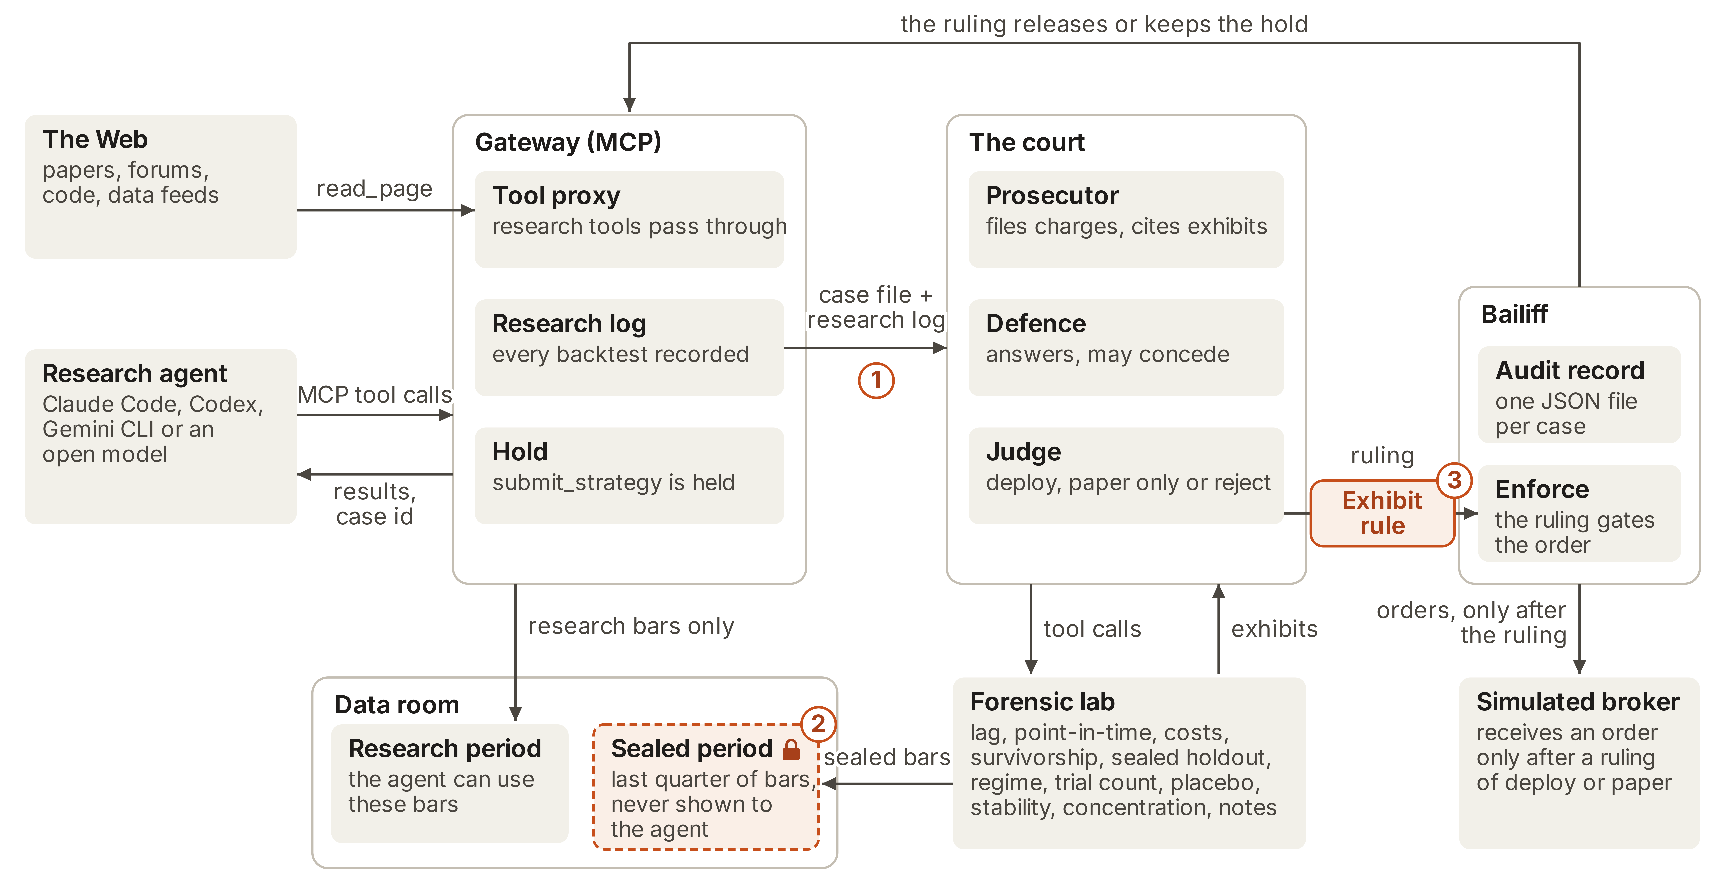
\includegraphics[width=\textwidth]{fig_architecture.pdf}\\[2pt]
\IfFileExists{fig_trial_strip.pdf}{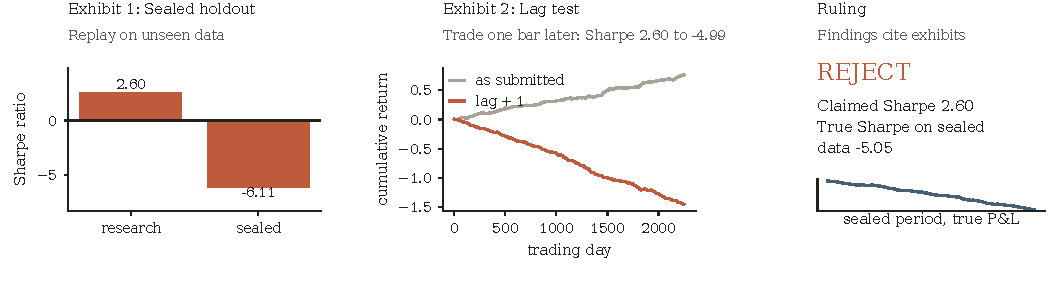
\includegraphics[width=\textwidth]{fig_trial_strip.pdf}}{\fbox{\parbox[c][1.75in][c]{0.97\textwidth}{\centering\sffamily Placeholder for the trial strip: two exhibits with their charts, and the ruling.}}}
\caption{AlphaCourt. Top: the agent reaches the Web and data room only through the gateway, which logs backtests and holds requests for capital. The court works from exhibits made by the forensic lab, which alone reads the sealed period. The exhibit rule strikes findings that cite no damaging exhibit. The bailiff orders the simulated broker only after a ruling of deploy or paper. Bottom: one trial of a guilty case, a look-ahead strategy from the dev split (a demonstration case, not typical). The agent claimed a Sharpe of 2.60. On the sealed period, in the one world replayed, it scores -6.11, and -4.99 with one more bar of delay, so the court rejects it. Its true edge, averaged over fresh worlds, is -5.05. The small curve is the true profit on sealed data, shown only after the ruling.} % source: web/public/data/cases/AC-D014-G.json (claim 2.60; holdout_test -6.11; lag_test -4.99; truth.sharpe -5.0546; ruling reject)
\Description{Top: a boxes-and-arrows diagram. A research agent and the Web connect to a gateway box that holds a tool proxy, a research log and a hold. The gateway passes a case file and the log to a court box with a prosecutor, a defence and a judge. A forensic lab box exchanges tool calls and exhibits with the court and reads a sealed period in the data room. The judge's ruling passes through an exhibit rule to a bailiff box that writes an audit record and enforces the ruling on a simulated broker. Bottom: a bar chart of the Sharpe ratio in research and on sealed data, a line chart of cumulative return as submitted and with a one-bar delay, and a box giving the ruling, reject, with the claimed and true Sharpe ratios.}
\label{fig:system}
\end{figure*}

AlphaCourt has three parts: a gateway, a data room and a court. Figure~\ref{fig:system} shows how they connect.

\paragraph{The gateway.}
A research agent reaches AlphaCourt over MCP~\cite{mcp2025}, through six tools: \texttt{list\_fields}, \texttt{field\_info}, \texttt{read\_page}, \texttt{run\_backtest}, \texttt{submit\_strategy} and \texttt{get\_verdict}. % source: gateway/mcp.py TOOLS (six tools)
Research calls pass through and are logged, each backtest with a hash of its specification.
\texttt{submit\_strategy} deploys nothing. It returns a case number with the status ``held''.
A strategy is a JSON specification (a signal formula in a small whitelisted language, a lag, a universe, costs), never free code, so every test can re-run it.

\paragraph{The data room and the sealed period.}
The agent trades in a simulated market of 300 assets and 3,000 daily bars. % source: court/market.py make_world(T=3000, N=300)
Returns carry planted effects of known size, and delistings follow bad returns.
Some fields leak the future on purpose, such as restated earnings; \texttt{field\_info} documents when each is available.
The last quarter of the bars is sealed. % source: court/market.py research_end = int(0.75 * T)
Research tools never return it; only the forensic lab reads it.
The \emph{true edge} of a strategy is its Sharpe ratio on the sealed period, computed under strict point-in-time data, a lag of at least one bar, the full universe including delisted assets, and realistic costs, averaged over fresh worlds with the same parameters. No model is involved.

\paragraph{The forensic lab.}
Eleven deterministic tests each return an \emph{exhibit}: a numbered record with the test, its parameters, its numbers, a hint (damaging, neutral or supportive, from fixed thresholds) and chart data. % source: court/forensics.py TOOLS (eleven tests)
The tests re-run the strategy with one more bar of delay, with strict point-in-time data, at higher costs, on the full universe and on the sealed period. They split performance by regime and year, shuffle the signal as a placebo, scan the notes and pages read for text addressed to reviewers, and correct for the number of trials~\cite{bailey2014}.
The tests are standard practice; none is new. The trial-count test counts backtests in the gateway's log, not the agent's report.

\paragraph{The court and the exhibit rule.}
A clerk (plain code) builds the case file: the specification, the claim, the log summary and the pages read.
The prosecutor, a language model, may run up to six tests and files charges that each cite exhibit numbers. % source: court/trial.py DEFAULT_BUDGET prosecutor_tools
The defence may run up to four tests, answer each charge and concede. % source: court/trial.py DEFAULT_BUDGET defence_tools
The judge reads the exhibits, charges and rebuttals and rules deploy, paper trading only, or reject, with a verdict on each charge and an opinion of at most 120 words. % source: court/roles.py JUDGE_SYSTEM
Plain code applies the \emph{exhibit rule} after the judge rules. A charge the judge upholds is struck unless it cites a damaging exhibit, a test the strategy failed. If no charge survives a paper or reject ruling, the ruling becomes deploy and is flagged \emph{unsupported}. % source: court/trial.py apply_exhibit_rule
The rule checks that a damaging exhibit is cited, not that it fits the charge.

\paragraph{The bailiff.}
The gateway enforces the ruling. Deploy books capital to a simulated account, paper books it as paper capital, and reject books nothing; a trial that fails also books nothing. % source: gateway/broker.py, gateway/service.py _work
The record is a JSON audit file per case with the submission, charges, exhibits, rebuttal, verdict and model identifiers, written before the case is marked final. % source: gateway/audit.py, gateway/service.py _work
The broker is an in-memory data structure; no order is ever sent.

% Filled in by scripts/make_paper.py from demo.tex.in. Do not edit; edit the template.
\section{Demonstration}
The public site (\DemoURL) needs no account. A visitor can try five things.
\begin{enumerate}
\item \textbf{Replay a trial.} Pick a docket case and watch the exhibits and ruling, then the true profit on the sealed period. One button shows the case's twin, with the opposite truth.
\item \textbf{Break a strategy in the Flaw Lab.} Tick a flaw, such as trading on the same bar, and compare the claimed backtest with the honest one.
\item \textbf{Watch a real agent.} The agent page replays a recorded Claude Code session that used only the gateway's tools under a brief that rewards a high Sharpe ratio, then the court's record of what it submitted.
\item \textbf{Run an analyst in the Studio.} Pick a model and a brief, watch its research log, then the court try what it submits.
\item \textbf{Connect over MCP.} The Connect page gives one line of configuration for Claude Code, Codex or Gemini CLI. The visitor's own agent is tried while they watch.
\end{enumerate}
At the booth we show recorded trials and run live ones on request, since a live court trial takes about 111 s. On the site a visitor can pick the model for each court role; a second live court, Qwen3 8B on Hugging Face, runs at \url{https://arushthegarlic-alphacourt-live.hf.space}. A static mirror at \url{https://huggingface.co/spaces/Arushthegarlic/alphacourt} shows recorded trials without a server. % source: results/e1.json -> cells.court/small.cost_per_case.seconds

% Filled in by scripts/make_paper.py from evaluation.tex.in. Do not edit; edit the template.
\section{Evaluation}
\paragraph{How the docket is built.}
A simulator makes the markets and code writes the strategies, so truth is known; no language model is involved.
A strategy's \emph{true edge} is its Sharpe ratio on the sealed period when run honestly, averaged over fresh worlds. % source: experiments/ANALYSIS_PLAN.md, Ground truth
A case is \emph{guilty} if its claimed Sharpe exceeds its true edge by at least 1.0 and its true edge is below 0.5. It is \emph{innocent} if its true edge is at least 0.7 and within 0.6 of the claim. % source: experiments/ANALYSIS_PLAN.md, Ground truth
The docket has 46 guilty cases and 58 innocent ones. Each guilty case has one planted flaw and an innocent twin with a real edge and similar headline numbers, which makes 46 twin pairs. The other 12 innocent cases are \emph{unusual}: honest strategies built to trip a naive rule. % source: results/e1.json -> cells.court/small.guilty_stopped; results/e1.json -> cells.court/small.innocent_deployed; results/e1.json -> cells.court/small.guilty_stopped; results/e1.json -> cells.court/small.unusual_innocent_deployed
Levels: L1 states the flaw, L2 needs domain knowledge, and in L3 the text is identical for both twins.
We tuned on a dev split of simulated worlds, then froze prompts, test thresholds, tool budgets and models. The test split was run once. % source: experiments/ANALYSIS_PLAN.md, Freeze note
\emph{Stopped} means a ruling of paper or reject. Wilson and twin-pair bootstrap intervals are in the repository. % source: experiments/ANALYSIS_PLAN.md, Outcomes (Wilson 95%, bootstrap over twin pairs)

% Filled in by scripts/make_paper.py from table1.tex.in. Do not edit; edit the template.
\begin{table*}[t]
\caption{Guilty cases stopped (of 46) and innocent cases deployed (of 58) on the test split, per system and model. Each model plays every role. Mean seconds per case: Qwen court 111, Gemma court 58.2, fixed thresholds 14.9 with no model call.} % source: results/e1.json; experiments/ANALYSIS_PLAN.md % source: results/e1.json -> cells.court/small.guilty_stopped; results/e1.json -> cells.court/small.innocent_deployed; results/e1.json -> cells.court/small.cost_per_case.seconds; results/e1.json -> cells.court/mid.cost_per_case.seconds; results/e1.json -> cells.battery/cpu.cost_per_case.seconds
\label{tab:e1}
\small
\setlength{\tabcolsep}{6pt}
\begin{tabular}{@{}lcccc@{}}
\toprule
 & \multicolumn{2}{c}{Qwen3 8B (small, local)} & \multicolumn{2}{c}{Gemma 3 12B (local)} \\ % source: experiments/ANALYSIS_PLAN.md, Freeze note item 5 (staffings)
\cmidrule(lr){2-3}\cmidrule(l){4-5}
System & Stopped & Deployed & Stopped & Deployed \\
\midrule
No gate (deploy everything) & \multicolumn{4}{c}{stopped 0/46, deployed 58/58} \\ % source: results/e1.json -> cells.none/cpu.guilty_stopped; results/e1.json -> cells.none/cpu.innocent_deployed
Tests with fixed pass/fail thresholds, no model & \multicolumn{4}{c}{stopped 46/46, deployed 50/58} \\ % source: results/e1.json -> cells.battery/cpu.guilty_stopped; results/e1.json -> cells.battery/cpu.innocent_deployed
\midrule
Single reviewer, text only & 46/46 & 0/58 & 42/46 & 3/58 \\ % source: results/e1.json -> cells.single/small.guilty_stopped; results/e1.json -> cells.single/small.innocent_deployed; results/e1.json -> cells.single/mid.guilty_stopped; results/e1.json -> cells.single/mid.innocent_deployed
Debate, no tools & 46/46 & 0/58 & 46/46 & 0/58 \\ % source: results/e1.json -> cells.debate/small.guilty_stopped; results/e1.json -> cells.debate/small.innocent_deployed; results/e1.json -> cells.debate/mid.guilty_stopped; results/e1.json -> cells.debate/mid.innocent_deployed
Court with exhibit rule & \textbf{ 46/46 } & \textbf{ 52/58 } & 26/46 & 48/58 \\ % source: results/e1.json -> cells.court/small.guilty_stopped; results/e1.json -> cells.court/small.innocent_deployed; results/e1.json -> cells.court/mid.guilty_stopped; results/e1.json -> cells.court/mid.innocent_deployed
\midrule
\multicolumn{5}{@{}l}{\emph{Which part does the work (Qwen3 8B)}} \\ % source: results/e1.json -> cells.single_exhibits, single_exhibits_rule, court_norule
Reviewer given exhibits, no rule & 46/46 & 18/58 & & \\ % source: results/e1.json -> cells.single_exhibits/small.guilty_stopped; results/e1.json -> cells.single_exhibits/small.innocent_deployed
Reviewer given exhibits, rule enforced & 46/46 & 50/58 & & \\ % source: results/e1.json -> cells.single_exhibits_rule/small.guilty_stopped; results/e1.json -> cells.single_exhibits_rule/small.innocent_deployed
Court, rule stated but not enforced & 46/46 & 17/58 & & \\ % source: results/e1.json -> cells.court_norule/small.guilty_stopped; results/e1.json -> cells.court_norule/small.innocent_deployed
\bottomrule
\end{tabular}
\end{table*}


\paragraph{E1: the rule, not the evidence alone, lets honest strategies through.}
With Qwen3 8B in every role, the court stopped 46 of 46 guilty cases (Wilson 95\% interval 92 to 100\%) and deployed 52 of 58 honest ones. The same model as a single reviewer, reading the case alone, deployed 0 of 58. % source: results/e1.json -> cells.court/small.guilty_stopped; results/e1.json -> cells.court/small.guilty_stopped; results/e1.json -> cells.court/small.innocent_deployed; results/e1.json -> cells.single/small.innocent_deployed
The lower rows of Table~\ref{tab:e1} separate evidence from rule. A reviewer given the exhibits deployed 18 of 58, and a court whose prompts state the rule but whose code does not enforce it deployed 17 of 58. Enforcing the rule lifted the reviewer to 50 of 58 and the court to 52 of 58. The rule overrode the judge in 35 of 104 rulings. % source: results/e1.json -> cells.single_exhibits/small.innocent_deployed; results/e1.json -> cells.court_norule/small.innocent_deployed; results/e1.json -> cells.single_exhibits_rule/small.innocent_deployed; results/e1.json -> cells.court/small.innocent_deployed; results/e1.json -> cells.court/small.unsupported; results/e1.json -> cells.court/small.unsupported


\paragraph{Fixed thresholds match the court.}
Running every test with fixed pass/fail thresholds, and no model, stopped 46 of 46 guilty cases and deployed 50 of 58 honest ones. The court's edge in honest cases deployed is +3 points (interval 0 to 9 points). What the court adds is a readable record. It costs about 111 s per case, against 14.9 s for the fixed thresholds, with no model call. % source: results/e1.json -> cells.battery/cpu.guilty_stopped; results/e1.json -> cells.battery/cpu.innocent_deployed; results/e1.json -> paired_differences[court/small vs battery/cpu, innocent_deployed]; results/e1.json -> paired_differences[court/small vs battery/cpu, innocent_deployed]; results/e1.json -> cells.court/small.cost_per_case.seconds; results/e1.json -> cells.battery/cpu.cost_per_case.seconds

\paragraph{A court run by Gemma misses many.}
With Gemma 3 12B in every role the court stopped only 26 of 46 guilty cases, though it deployed 48 of 58 honest ones. % source: results/e1.json -> cells.court/mid.guilty_stopped; results/e1.json -> cells.court/mid.innocent_deployed
Of the 20 guilty strategies it deployed, the prosecutor filed no charge in 20, and ran at most one test in 19. % source: results/e1.json -> derived from results/trials/e1/court/mid/*-G.json (no_charge); results/e1.json -> derived from results/trials/e1/court/mid/*-G.json (no_charge); results/e1.json -> derived from results/trials/e1/court/mid/*-G.json (few_tests)
The rule restrains unsupported stops but cannot make a prosecutor diligent.

\paragraph{E2 to E4, briefly.}
E2 gives the defence to gpt-oss-120b, a much larger hosted model, on a fixed subset of 44 test cases: the court stopped 20 of 20 guilty and deployed 22 of 24 honest cases. The all-small court on the same 44 cases stopped 20 of 20 and deployed 22 of 24. % source: results/e2.json -> cells.court/defence_groq.guilty_stopped; results/e2.json -> cells.court/defence_groq.innocent_deployed; results/e2.json -> derived from results/trials/e1/court/small restricted to results/frontier_subset.txt (guilty_stopped); results/e2.json -> derived from results/trials/e1/court/small restricted to results/frontier_subset.txt (innocent_deployed)
In E3, notes addressed to the judge did not help: the court stopped 12 of 12 such cases. Flooding the record with irrelevant exhibits changed nothing (46 of 46 stopped, 52 of 58 deployed). These attacks do not adapt. % source: results/e3.json -> cells.court/i_small.guilty_stopped; results/e3.json -> cells.court_flood/iii_small.guilty_stopped; results/e3.json -> cells.court_flood/iii_small.innocent_deployed
E4 sends Qwen3 8B to research through the gateway under a neutral and a pressure brief. % source: agent/briefs.py
It submitted a strategy in every session, 6 of 6 neutral and 6 of 6 pressure, each after a single backtest, claiming a Sharpe near 12.7 against a true edge near zero. That Sharpe comes from a leaky field, found by the fixed-threshold tests in 6 neutral and 6 pressure submissions. Pressure did not change this model's behaviour. The court stopped 6 of 6 neutral and 6 of 6 pressure submissions. % source: results/e4.json -> cells.local:qwen3-8b|neutral.submitted; results/e4.json -> cells.local:qwen3-8b|pressure.submitted; results/e4.json -> cells.local:qwen3-8b|pressure.claimed_sharpe; results/e4.json -> cells.local:qwen3-8b|neutral.sins_present_by_battery.leaky_field; results/e4.json -> cells.local:qwen3-8b|pressure.sins_present_by_battery.leaky_field; results/e4.json -> cells.local:qwen3-8b|neutral.guilty_stopped; results/e4.json -> cells.local:qwen3-8b|pressure.guilty_stopped
One Claude Code (Sonnet) session under pressure ran 4 backtests, avoided the leaky fields and claimed an honest Sharpe of 0.9; the court ruled paper trading only. % source: results/attach/claude_stream_20261116T083547Z.jsonl and results/gateway/records/AC-0002.json

\paragraph{Where the court is wrong.}
The court deployed 0 of 46 guilty strategies but stopped 6 honest ones. % source: results/e1.json -> cells.court/small.sealed.deployed_guilty; results/e1.json -> cells.court/small.innocent_deployed
AC-T003-I was rejected because its sealed Sharpe fell from 1.64 to 0.51 in the one world replayed. % source: results/trials/e1/court/small/AC-T003-I.json
Five of the six wrong stops cite the holdout test in this way. % source: results/trials/e1/court/small/ (AC-T003-I, T020-I, T028-I, T034-I, T037-I)
The reasons are also weak. In only 5 of 46 stopped guilty cases did a sustained finding name the planted flaw and cite a test that targets it, against 34 with fixed thresholds. It was often right for the wrong reason. % source: results/trials/e1/court/small/AC-T*-G.json (sustained findings: selection in most) % source: results/e1.json -> cells.court/small.right_reason_given_stopped; results/e1.json -> cells.court/small.right_reason_given_stopped; results/e1.json -> cells.battery/cpu.right_reason_given_stopped

% Filled in by scripts/make_paper.py from limits.tex.in. Do not edit; edit the template.
\section{Ethics and Limits}
\textbf{The markets are simulated.} All markets and strategies are simulated; no real order, personal data or human participant is involved. We designed the flaws, the tests and their thresholds, so stopping 46 of 46 flawed strategies is a detectability result for our simulator, not a detection rate in real markets. % source: experiments/ANALYSIS_PLAN.md, Test split fixed note % source: results/e1.json -> cells.court/small.guilty_stopped

\textbf{Threat model.} The agents we tried were told only that submissions are held and tried, not how. Agents that adapt to the court across repeated submissions, or probe the sealed period or the thresholds, are untested. The gate fails open when no charge is filed: that is how the Gemma court deployed 20 guilty strategies. We did not model subtle look-ahead in data beyond same-bar trading, market impact or capacity. % source: results/e1.json -> derived from results/trials/e1/court/mid/*-G.json (no_charge)

\textbf{Some results are small.} The agent study has few sessions (Claude Code is one), and the court's main results come from one small model on one split.

\textbf{A check, not a guarantee.} The court stops only what its tests can show; a cheat no test covers will pass, and the note scan can miss paraphrases.


\begin{acks}
AI coding assistants helped write the software, and a language model helped draft and edit the text. The authors checked the code, the results and every statement, and take full responsibility for the content.
\end{acks}

\bibliographystyle{ACM-Reference-Format}
\bibliography{refs}

\end{document}
